
\section{Voice Recognition}

\subsection{Algorithm Used}
\begin{enumerate}
  \item An utterance of a user is collected during the enrollment procedure.
  \item Voice Activity Detection is performed: Signals must be first filtered to rule out the silence part, otherwise the training might be seriously biased.
  \item Feature Extraction
    \begin{itemize}
      \item Mel-Frequency Cepstral Coefficient (MFCC) is a representation of the short term power spectrum of a sound, based on a linear cosine transform of a log power spectrum on a non-linear mel-scale of frequency . MFCC is the most widely used features in Automatic Speech Recognition, and it can also be applied to speaker recognition task. The process to extract MFCC feature is demonstrated in Figure \ref{fig:MFCC_fig_one}. \\
      %\begin{figure}[!t]
      %\centering
      %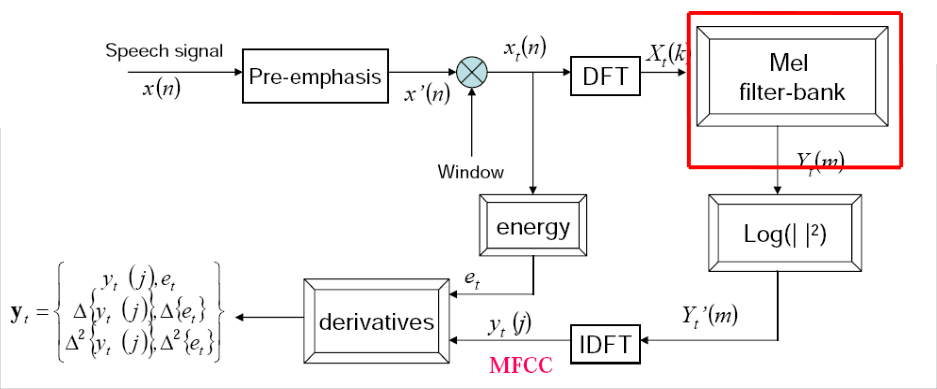
\includegraphics[width=2.5in]{./MFCC-mel-filterbank.png}
      % where an .eps filename suffix will be assumed under latex,
      % and a .pdf suffix will be assumed for pdflatex; or what has been declared
      % via \DeclareGraphicsExtensions.
      %\caption{MFCC Feature Extraction Process}
      %\label{fig:MFCC_fig_one}
      %\end{figure}
      \\
      \item Linear Predictive Coding (LPC) is a tool used in audio signal processing and speech processing for representing the spectral envelope of a digital signal of speech in compressed form, using the information of a Linear predictive Model. \\
      The basic assumption in LPC is that, the n th signal is a linear combination of the previous p signals. Therefore, to estimate the coefficients ai, we have to minimize the squared error. This optimization can be done by Levinson-Durbin algorithm.
    \end{itemize}
  \item Gaussian Mixture Model (GMM) is used in acoustic learning task such as speaker recognition, since it describes the varied distribution of all the feature vectors. Therefore, GMM is merely a weighted combination of multivariate Gaussian distribution which assumes feature vectors are independent. We use diagonal covariance since the dimensions of the feature vector is independent to each other. GMM can describe the distribution of feature vector with several clusters, as shown in Figure \ref{fig:GMM_fig_one}. \\
  \begin{figure}[!t]
  \centering
  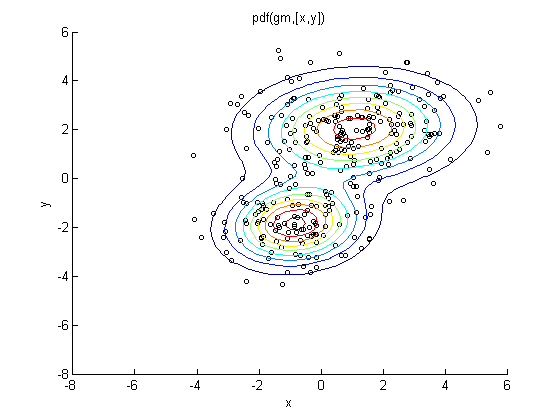
\includegraphics[width=2.5in]{./gmm.png}
  % where an .eps filename suffix will be assumed under latex,
  % and a .pdf suffix will be assumed for pdflatex; or what has been declared
  % via \DeclareGraphicsExtensions.
  \caption{A Two Dimensional GMM with Two Components}
  \label{fig:GMM_fig_one}
  \end{figure}
  \\
  After training, the model can give the score of fitness for every input feature vector, measuring the probability that the vector belongs to this model. Therefore in the task of speaker recognition, we can train a GMM for every speaker. Then for a input signal, we extract lists of feature vectors for it, and calculate the overall likelihood that the vector belongs to each model. The speaker whose model fits the input best will be chosen as the answer. \\
  Moreover, an enhancement has been done to the original GMM method. The training of GMM first requires a random initialization of the means of all the components. However, we can first use K-means algorithm to perform a clustering to all the vectors, then use the clustered centers to initialize the training of GMM. This enhancement can speed up the training and also give a better training result.
  \item Joint Factor Analysis (JFA) is a typical method which behave very well in classification problems, due to its ability to account for different types of variability in training data. Within all the factor analysis methods, JFA was proved to outperform other methods in the task of speaker recognition. \\  JFA models the user by supervector, i.e., a C x F dimension vector, where C is the number of components in the Universal Background Model, trained by GMM on all the training data, and F is the dimension of the acoustic feature vector. The supervector of an utterance is obtained by concatenating all the C means vectors in the trained GMM model.
\end{enumerate}
